\documentclass{beamer}

\usetheme{Szeged}

\usepackage{amssymb,amsmath,mathrsfs}
\usepackage{catchfile,etoolbox}
\usepackage{subfig}
\usepackage{epsfig,psfrag}
\usepackage[update]{epstopdf}

\usepackage{xspace}

\usepackage{graphicx}
\graphicspath{{figs/}}
\DeclareGraphicsExtensions{.pdf,.eps,.jpg,.png}

\usepackage{media9}
\addmediapath{videos}

\usepackage{gamm}

\title[Energy Shaping]{Optimal Energy-Based Control of Hybrid Systems}
\subtitle{with Applications to Robotic Walking}
\author{\emph{Ryan W. Sinnet} and Aaron D. Ames}
\institute{Department of Mechanical Engineering\\ Texas A\&M University}
\date{Monday, March 23, 2015}

\makeatletter
\def\input@path{{figs/}{sections/}}
\makeatother

\begin{document}

\frame{\titlepage}


% motivation for energy shaping
% explanation as optimal controller
% slack variables for practical implementations
% cart--spring system

\section{Introduction}
\showtoc

\subsection{Motivation}

\begin{frame}[t]
  \frametitle{Motivation}
  \only<1> {
    \begin{block}{Goal}
      Design an optimal controller to shape the energy dynamics of periodic
      behaviors in mechanical systems without destroying stability.
    \end{block}

    \begin{block}{Considerations}
      \begin{itemize}
      \item Should work on systems with impulse effects
      \item Should be computationally tractable
      \item Should not alter the steady-state periodic behavior
      \item Control law should be guaranteed to exist at least locally
      \end{itemize}
    \end{block}
  }

  \only<2>{
    \begin{block}{Problem}
      Certain controllers induce periodic behaviors \red{but}
      altering gains can change overall trajectory.
    \end{block}
      
    \begin{block}{Question}
      How can we make such controllers more robust without altering the
      steady-state behavior?
    \end{block}

    \begin{block}{Solution}
      Take advantage of the periodic nature of energy to stabilize the energy
      dynamics.
    \end{block}
  }
\end{frame}

\begin{frame}[t]
  \frametitle{Existing Results}
  \begin{block}{Total Energy Shaping and controlled symmetries}
    \small
    M. W. Spong, J. K. Holm, and D. Lee. {\em Passivity-based control of
      bipedal locomotion}. IEEE T. Robotic. Autom., 14(2), pp.~30--40,
    2007.
  \end{block}
  \begin{block}{Controlled Lagrangians}
    \small
    A. M. Bloch, N. E. Leonard and J.E. Marsden. {\em Controlled Lagrangians
      and the stabilization of mechanical systems I: The first matching
      theorem}. IEEE T. Automat. Contr., 45(12), pp.~2253--2270, 2000.
  \end{block}
  \begin{block}{Rapidly exponentially stabilizing control Lyapunov functions}
    \small
    A. D. Ames, K. Galloway, K. Sreenath, and J. W. Grizzle. {\em Rapidly
    exponentially stabilizing control Lyapunov functions and hybrid zero
    dynamics}. IEEE T. Automat. Contr., 59(4), pp.~876--891, 2014.
  \end{block}

\end{frame}
\section{Mechanics}
\showtoc

\subsection{Hybrid Systems}
\begin{frame}[t]
  \frametitle{Bipedal Models}
  \begin{figure}
    \centering
    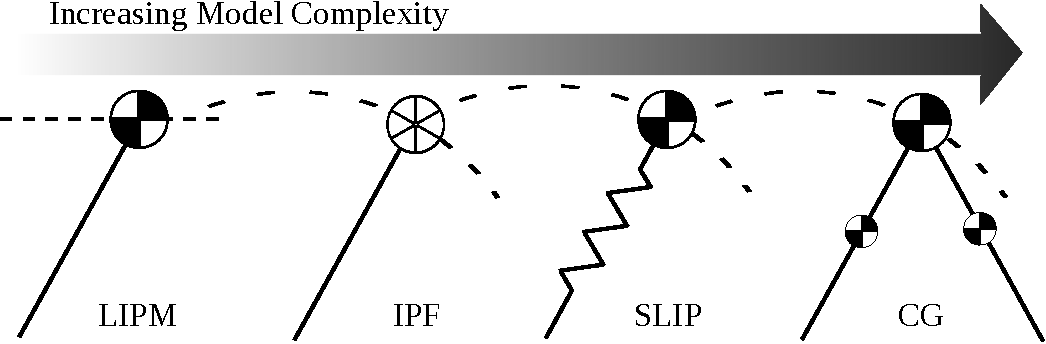
\includegraphics[width=.9\textwidth]{biped-models}
  \end{figure}
  \begin{itemize}
  \item Bipedal locomotion has been studied with a variety of models.
  \item Pendulum models consider massless legs with no impacts.
  \item Kinematic chains are markedly more complex than pendula.
  \end{itemize}
\end{frame}

\begin{frame}[t]
  \frametitle{Modeling Hybrid Systems}
  \begin{columns}
    \begin{column}{.63\textwidth}
      \begin{definition}
        A \alert{hybrid control system} is a tuple \vspace{-.3cm}
        $$\HCS = \hcsystem, \vspace{-.4cm}$$
        where
        \begin{itemize}
        \item
          $\Domain \subset \X$ is the \blue{domain of admissibility} with state space $\X$,
        \item
          $\ControlSet$ is a set of \blue{admissible controls},
        \item
          $\Guard$ is a \blue{guard} or \blue{switching surface},
        \item
          $\ResetMap$ is a smooth \blue{reset map},
        \item
          $(\xf, \xg)$ is a \blue{control system} on $\Domain$: \vspace{-3mm}
          \begin{align*}
            \dx = \xf(\x) + \xg(\x) \, \uu.
          \end{align*}
        \end{itemize}
      \end{definition}
    \end{column}
    \begin{column}{.4\textwidth}
      \begin{figure}    
        \centering
        \def\svgwidth{.8\columnwidth}
        \input{figs/simple_hybrid_system.eps_latex}
      \end{figure}
      \vspace{-1em}
      A \alert{simple hybrid system}:\vspace{-.5em}
      $$\HS = \hsystem$$
    \end{column}
  \end{columns}
\end{frame}

\begin{frame}[t]
  \frametitle{Lagrangian Systems}
  Mechanical systems are defined by:
  \begin{itemize}
  \item Kinetic energy, $T : T\sQ \to \Rnn$,\\
  \item Potential energy, $U : \sQ \to \R$,
  \end{itemize}
  which together comprise the Lagrangian,
  \begin{align*}
    \Lagrangian\argsqdq = T\argsqdq - U\argsqdq.
  \end{align*}
  Dynamical motion in such a system with external forcing $\mathcal{F} = B\argsq u$ is governed by the Euler--Lagrange equation:
  \begin{align*}
    \frac{d}{dt} \pd{\Lagrangian}{\dq} - \pd{\Lagrangian}{\q} = B\argsq u.
  \end{align*}
\end{frame}

\begin{frame}[t]

  \frametitle{Swing Phase Dynamics}
  \begin{columns}
    \begin{column}{.55\textwidth}
      For Lagrangian $\Lagrangian$ with coordinates
      \begin{align*}
        \x = \argsqdq \in T\ConfigurationSpace,
      \end{align*}
      the dynamic model has the form
      \begin{align*}
        \M\argsq \, \ddq + \C\argsqdq \, \dq + \G\argsq = \B\argsq \, \uu,
      \end{align*}
      or $\dx = \xf\argsqdq+ \xg\argsq \, \uu,$ with
      \begin{align*}
        \xf\argsqdq &= \left(\!\!\begin{array}{c}
            \dq\\
            \M^{-1}\argsq (-\C\argsqdq \, \dq - \G\argsq)
          \end{array}\!\!\right),\\
        \xg(\q) &= \left(\!\!\begin{array}{c}
            \mathbf{0}_{m \times m}\\
            \M^{-1}(\q) \B(\q)
          \end{array}\!\!\right).
      \end{align*}
    \end{column}\!\!
    \begin{column}{.45\textwidth}
      \begin{figure}
        \centering
        \vspace{-10mm}
        \caption{Physical configuration}
        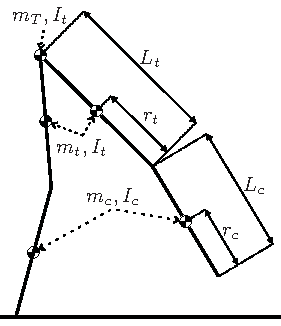
\includegraphics[width = 1.0\columnwidth]{pointfoot_robot_config}
      \end{figure}
    \end{column}
  \end{columns}
\end{frame}

\begin{frame}[t]
  \frametitle{Impact Dynamics}
  Introduce extended coordinates $\qe = (X, \q) \in \mathrm{SE}(3) \times \ConfigurationSpace$ which contains the kinematics of a reference point on the robot. Angular momentum balance based on H{\"u}rm{\"u}zl{\"u} and Marghitu:
  \begin{massump}
    \vspace{-.3em}
    \begin{itemize}
    \item Rigid-body plastic impacts with no slipping or rebounding
    \item Motors do not produce impulses
    \item No instantaneous change in configuration, i.e., $\qe^{-} = \qe^{+}$
    \end{itemize}
  \end{massump}\vspace{-.5em}
  Under these assumptions, the discrete dynamics satisfies
  \begin{align*}
    \left[\begin{array}{c c}
        \D_{e}(\qe) & -\Jacobian^{T}(\qe)\\
        \Jacobian(\qe) & \mathbf{0}_{3 \times 3}
      \end{array}\right]
    \left[\begin{array}{c}
        \dq^{+}\\
        \delta F(\qe, \dqe)
      \end{array}\right]
    = \left[\begin{array}{c c}
        \D_{e}(\qe) \, \dqe^{-}\\
        \mathbf{0}_{3}
      \end{array}\right].
  \end{align*}
\end{frame}

\subsection{Solutions to Hybrid Systems}
\begin{frame}[t]
  \frametitle{Hybrid Flows}
  A \alert{hybrid flow} of $\HS$ is a tuple
  \begin{align*}
    \chi^{\HS} = \left( \Delta, \mathscr{I}, \mathscr{C} \right),
  \end{align*}
  \vspace{-2em}
  \begin{itemize}
  \item $\Delta = \{0, 1, 2, \ldots\} \subseteq \Nat$ is a finite or infinite \blue{indexing set},
  \item $\mathscr{I} = \{I_{i} \}_{i \in \Delta}$ is a \blue{hybrid interval} where $I_{i} = [\tau_{i}, \tau_{i + 1}]$,
  \item $\mathscr{C} = \{c_{i} \}_{i \in \Delta}$ is a \blue{collection of solutions} of $\xf$, i.e., ${\dot c}_{i}(t) = \xf(c_{i}(t))$ $\forall i \in \Delta$.
  \end{itemize}

  \only<1>{
    \vspace{-1em}
    \begin{figure}
      \centering
      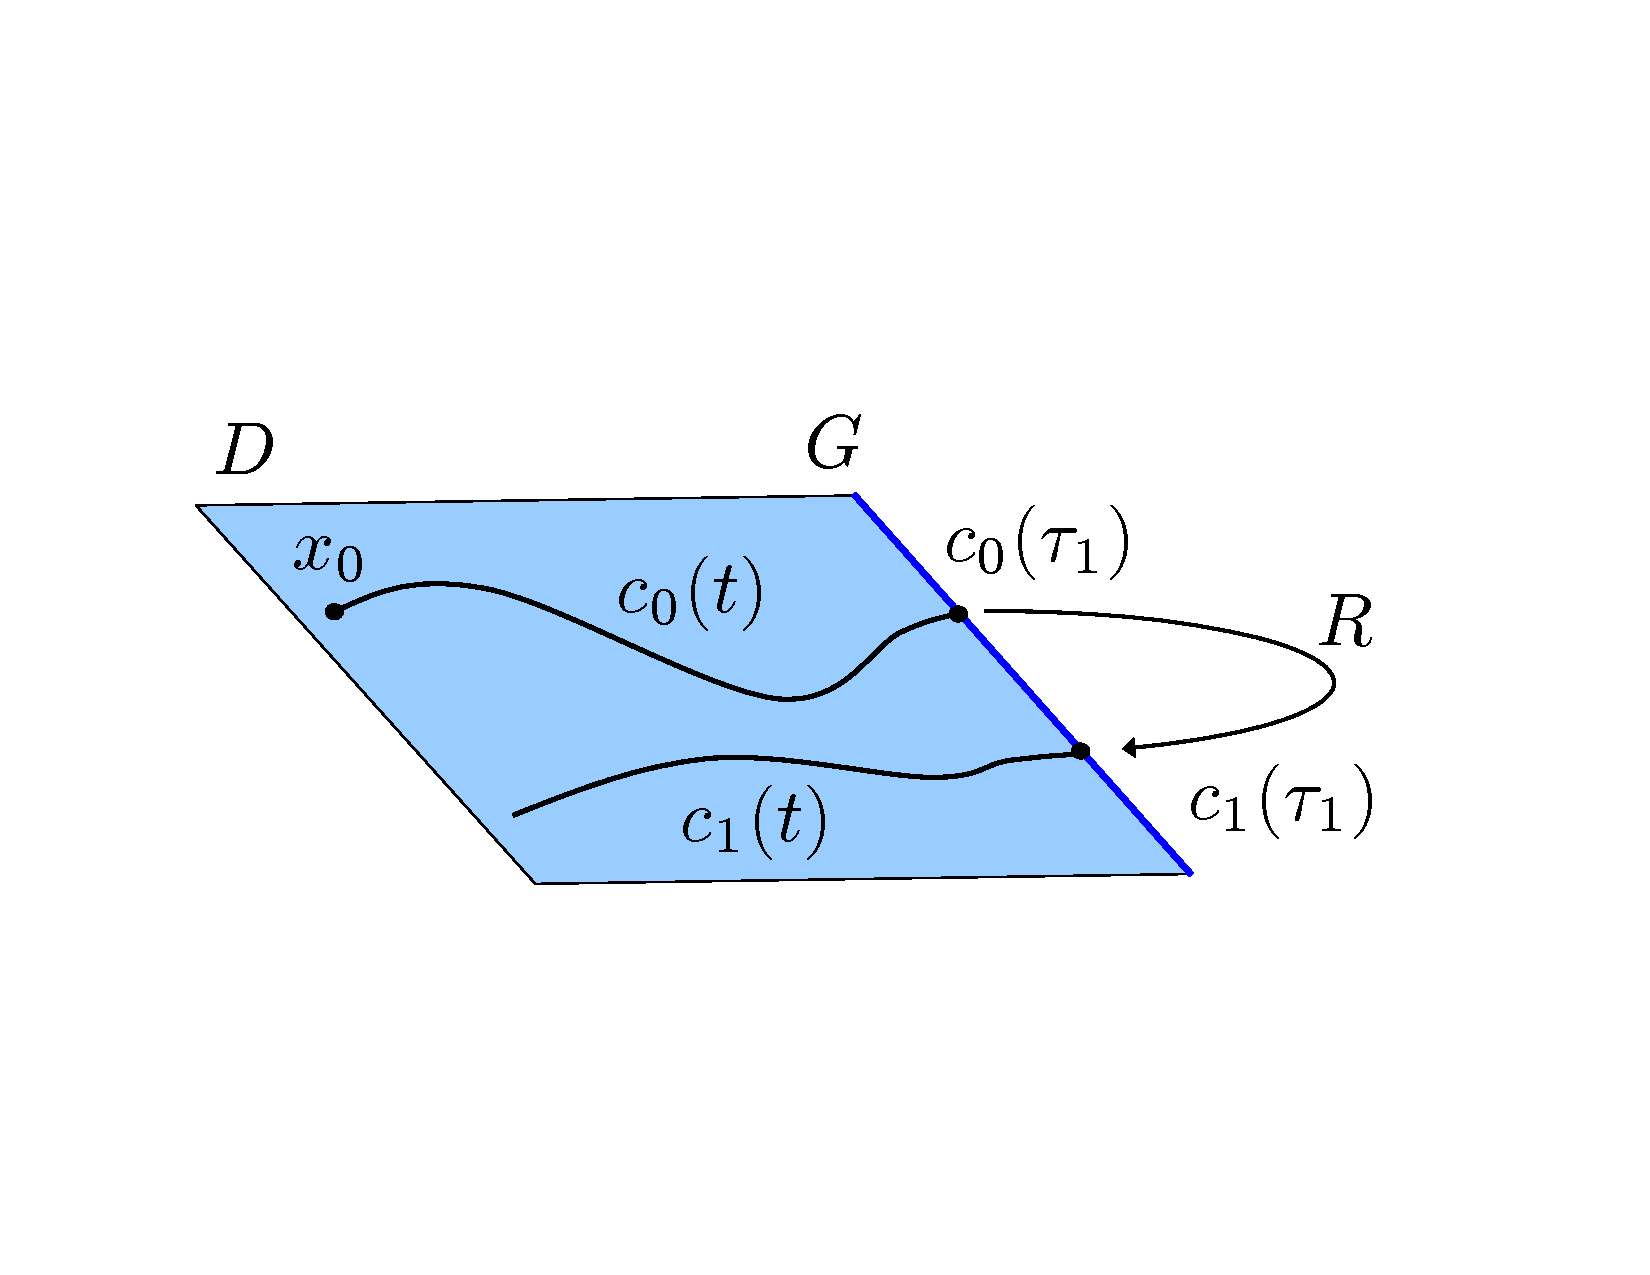
\includegraphics[width=0.5\columnwidth]{hybridflow}
    \end{figure}
    \vspace{-1em}
  }

  \only<2>{
    In addition, for every $i, i + 1 \in \Delta$, it is required that
    \begin{enumerate}
    \item $c_{i}(\tau_{i+1}) \in G$ and
    \item $\Delta(c_{i}(\tau_{i+1})) = c_{i+1}(\tau_{i+1})$
    \end{enumerate}
  }
\end{frame}


\begin{frame}[t]
  \frametitle{Periodic Orbits}
  \begin{figure}    
    \centering
    \def\svgwidth{.45\columnwidth}
    \input{figs/hybrid_periodic_orbit.eps_latex}
    \caption{A hybrid periodic orbit. Stability is ascertained using the method of Poincar\'e.}
  \end{figure}
\end{frame}

\begin{frame}[t]
  \frametitle{Conservative Systems}
  For a conservative system, total energy is conserved; i.e.:
  \begin{align*}
    \Ec &= T\argsqdq + U\argsq\\
    &= \E(q(0), \dot q(0)) = \E_{0}
  \end{align*}
  Dynamical motion for such a system relies on the interplay between kinetic and potential energy, which is expressed in the Euler-Lagrange equation,
  \begin{align*}
    \frac{d}{dt} \pd{\Lagrangian}{\dq} - \pd{\Lagrangian}{\q} = 0.
  \end{align*}
\end{frame}


\begin{frame}[t]
  \frametitle{The Simplest Example: Passive Compass-Gait Biped}
  \only<1>{
    \begin{columns}
      \column{1.5in}
      Dynamic Model:
      \begin{align*}
        \M\argsq \ddot q + \CG\argsqdq = 0
      \end{align*}
      Control Law:
      \begin{align*}
        \uu = 0.
      \end{align*}
      \column{1.5in}
      \begin{figure}%width=1.0\columnwidth,
        
        \centering
        \def\svgwidth{1.0\columnwidth}
        \input{figs/cg2d-slope-model.eps_latex}
        \vspace{-2em}
        \caption{Compass-gait biped falling down a slope.}
      \end{figure}
    \end{columns}
  }

  \only<2>{
    \begin{figure}
      \includemedia[
      % width=1.0\columnwidth,
      % height=0.5625\columnwidth,
      %width=1.0\columnwidth,
      %height=0.5\columnwidth,
      width=.9\columnwidth,
      height=0.45\columnwidth,
      addresource=cg2d_slope.mp4,
      activate=pageopen,
      flashvars={source=cg2d_slope.mp4&loop=true&autoPlay=true}
      ]{}{VPlayer9.swf}
      \caption{Stable passive gaits can be found for a range of slopes.}
    \end{figure}    
  }

  \only<3>{
    \begin{figure}
      \centering
      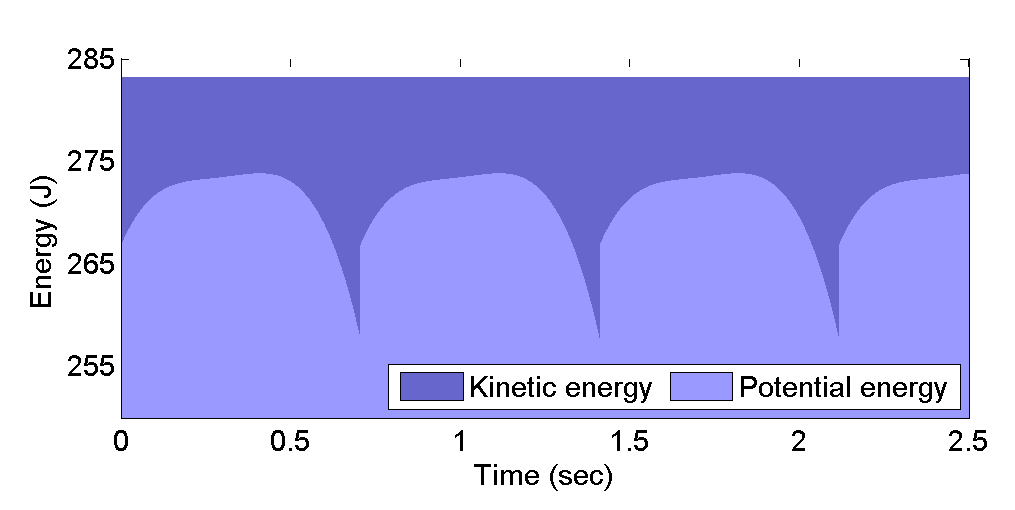
\includegraphics[width=1.0\columnwidth]{energy_cg2d_slope_model}
      \caption{Energy is exchanged between kinetic and potential in form.}
    \end{figure}    
  }
\end{frame}


\begin{frame}[t]
  \frametitle{Nonconservative Systems}
  For a nonconservative system, energy flows out of the system at a rate of $F_{\nc} \cdot dq$. Thus, the following quantity is conserved:
  \begin{align*}
    \Ec &= T\argsqdq + U\argsq - \int_{t_{0}}^{t} \! F_{\nc} \cdot \frac{dq}{d\tau} \ d\tau\\
    &= \E(q(0), \dot q(0)) = \E_{0}
  \end{align*}
  This equation expresses the interplay between kinetic and potential energy and the flow of energy into and out of the system.
\end{frame}


\begin{frame}[t]
  \frametitle{Example: 3-Link Biped}
  \only<1>{
    \begin{columns}
      \column{1.5in}
      Dynamic Model:
      \begin{align*}
        \M\argsq \ddq + \CG\argsqdq = \B\argsq \uu
      \end{align*}
      Control Law:
      \begin{align*}
        \uu &= \G\argsq - \G(\Psi\argsq)\\
        \uu_3 &=-k_{d} (\dot \vartheta_{T}^{a})\\
        &\hspace{1.8em} -k_{p} (\vartheta_{T}^{a} - \vartheta_{T}^{d})
      \end{align*}
      \column{1.5in}
      \begin{figure}
        \centering
        \def\svgwidth{1.0\columnwidth}
        \input{figs/cg2d-3link-model.eps_latex}
        \vspace{-2em}
        \caption{3-link biped configuration.}
      \end{figure}
    \end{columns}
  }

  \only<2>{
    \begin{figure}
      \centering
      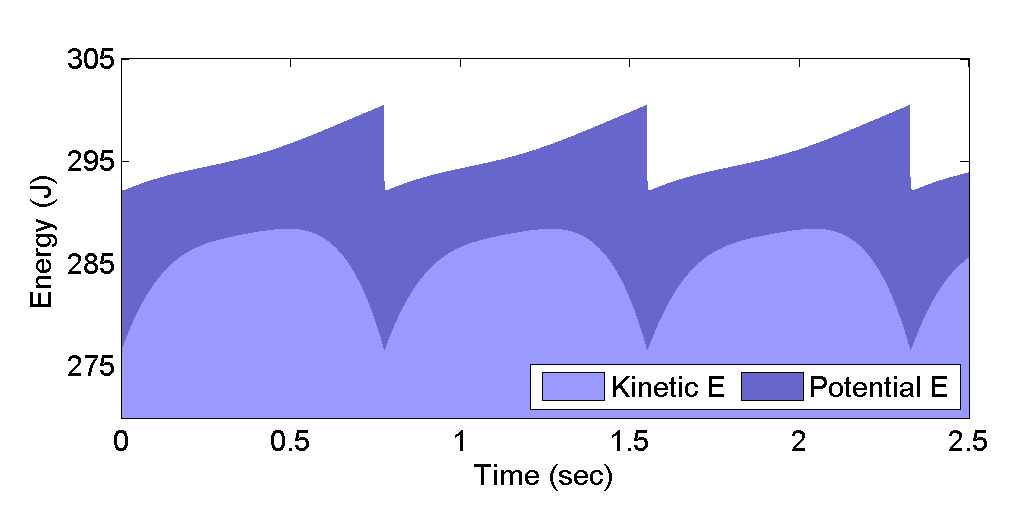
\includegraphics[width=1.0\columnwidth]{energy_cg2d_3link}
      \caption{Energy is not conserved as the controller injects energy.}
    \end{figure}
  }

  \only<3>{
    \begin{figure}
      \includemedia[
      %width=1.0\columnwidth,
      %height=0.5\columnwidth,
      width=.9\columnwidth,
      height=0.45\columnwidth,
      addresource=cg2d_3link_simulation.mp4,
      activate=pageopen,
      flashvars={source=cg2d_3link_simulation.mp4&loop=true&autoPlay=true}
      ]{}{VPlayer9.swf}
      \caption{Stable passive gaits can be found for a range of slopes.}
    \end{figure}
  }
\end{frame}

\section{Energy Shaping}
\showtoc

\subsection{Energy Shaping with Control Lyapunov Functions}

\begin{frame}[t]
  \frametitle{Motivation}
  \begin{block}{Main Question}
    Can we use an understanding of energy exchange to improve robustness  of
    periodic orbits in hybrid mechanical systems?
  \end{block}

  \begin{block}{Observations}
    \begin{itemize}
    \item Numerous control design schemes exist for stabilizing hybrid mechanical
      systems to periodic orbits.
    \item Some controllers produce good behavior locally but lack robustness.
    \item Periodic orbits have associated energy functions with level sets which
      are invariant under the orbits.
    \end{itemize}
  \end{block}
\end{frame}

\begin{frame}[t]
  \frametitle{Overview}
  \begin{block}{Main Idea}
    Add robustness to a periodic behavior by imposing convergence on a conserved
    energy function, $\Ec : \x \to \R$, to a level set which is known to be
    invariant under the system dynamics.
  \end{block}
  
  \begin{block}{Control Objective}
    Choose control input $\mu\arx$ such that $\| \mu\arx \|$ is minimized and
    $\Ec\arxt \to \Eref$ as $t \to \infty$.
  \end{block}

  \begin{block}{Exponential Convergence}
    To achieve exponential stabilization, $\Ec\arxt$ should satisfy\vspace{-.4em}
    \begin{align*}
      \Ec\arxt \leq \Ec\arxzero e^{-\beta t} \mbox{ for } t \geq 0, \beta > 0.
    \end{align*}
  \end{block}
\end{frame}

\begin{frame}[t]
  \frametitle{Conserved Energy Functions}
  \only<1> {
    \begin{block}{Conservative Systems}
      A conservative system with state space $\x = \argsqdq$ is modeled as
      \begin{align*}
        \HCSbar = \left\{
          \begin{array}{l l}
            \left.\begin{array}{r c l}
                \hspace{.58em}\dx &=& \xfbar\argsqdq + \xgbar\argsq \, \uu
              \end{array}\right\}  & \mbox{if } \argsqdq \in \D \setminus \S,\\
            \left. \begin{array}{r c l}
                \qp &=& \Deltaq\argsqm\\
                \dqp &=& \Deltadq\argsqdqm
              \end{array} \right\} & \mbox{if } \argsqdq \in \S,
          \end{array}\right.
      \end{align*}
      where $\xfbar\argsqdq := \xf\argsqdq$ and $\xgbar\argsq := \xg\argsq$ for
      notational clarity. Total energy is conserved through the continuous
      dynamics, i.e.,
      \begin{align*}
        \Ec\argsqdq := \Tnrg\argsqdq + \Unrg\argsq.
      \end{align*}
    \end{block}
  }

  \only<2> {
    \begin{block}{Nonconservative Systems}
      To properly handle the flow of energy due to $\vv\argsqdq$, define a storage
      function, \W, which obeys the differential equation
      \begin{align*}
        d\W = \vfR\argsqdq \, dt = \left( \B\argsq \, \vv\argsqdq \right)^{T}
        \frac{d\q}{dt}\art \, dt.
      \end{align*}
      Using \W, augment the state space, i.e., $\x := (\q, \dq, \W)$, and the vector
      fields (subsuming $\vv\argsqdq$ under $\xfbar\argsqdq$), i.e, 
      \begin{align*}
        \xfbar\argsqdq := \left(\begin{array}{c}
            \xf\argsqdq + \xg\argsq \, \vv\argsqdq\\
            \vfR\argsqdq
          \end{array}\right), &&
        \xgbar\argsq := \left(\begin{array}{c}
            \xg\argsq\\
            \boldzero
          \end{array}\right).
      \end{align*}
    \end{block}
  }
  \only<3> {
    \begin{block}{Nonconservative Systems}
      Use the augmented state to define the hybrid control system
      \begin{align*}
        \HCSbar = \left\{
          \begin{array}{l l}
            \left.\begin{array}{r c l}
                \hspace{1.15em}\dx &=& \xfbar\argsqdq + \xgbar\argsq \, \uu
              \end{array}\right\}  & \mbox{if } \argsqdq \in \D \setminus \S,\\
            \left. \begin{array}{r c l}
                \qp &=& \Deltaq\argsqm\\
                \dqp &=& \Deltadq\argsqdqm\\
                \Wp &=& \DeltaW = 0
              \end{array} \right\} & \mbox{if } \argsqdq \in \S.
          \end{array}\right.
      \end{align*}
      For such a system, the following quantity is conserved:
      \begin{align*}
        \Ec\argsqdqW := \Tnrg\argsqdq + \Unrg\argsq - W.
      \end{align*}
    \end{block}
  }
\end{frame}

\begin{frame}[t]
  \frametitle{Rapidly Exponentially Stabilizing CLFs}
  A \blue{rapidly exponentially stability control Lyapunov function (\RESCLF)}
  $\Ve : \X \to \Rnn$ satisfies
  \begin{align*}
    &\cc_{1} \nx^{2} \leq \Ve\arx \leq \frac{\cc_{2}}{\resclfparam^{2}} \nx^{2},\\
    &\inf_{\uu \in \U} \Lie{\xfbar}\Ve\arx + \Lie{\xgbar}\Ve\arx \, \uu +
    \frac{\cc_{3}}{\resclfparam} \Ve\arx \leq 0
  \end{align*}
  for $\cc_{1}, \cc_{2}, \cc_{3} > 0$ exhibits exponential convergence. If the above
  are satisfied, then it is also true that
  \begin{align*}
    \left\| \pd{\Ve\arx}{\x} \right\| \leq \cc_{4} \nx.
  \end{align*}
\end{frame}

\begin{frame}[t]
  \frametitle{Energy Shaping}
  Consider a conserved energy function $\Ec\arx$ on a hybrid control system
  \HCSbar which has a periodic orbit \orbit and define a Lyapunov candidate:
  \begin{align*}
    V\arx = \frac{1}{2} \left(\Ec\arx - \Eref\right)^{2},
  \end{align*}
  with $\Eref$ the constant energy level of the system on the orbit
  \orbit. For a \RESCLF, we seek a feedback control law, $\mu\arx$, such that
  \begin{align*}
    \Lie{\xfbar} V\arx + \Lie{\xgbar} \V\arx \, \mu\arx + \epsilon \V\arx &\leq 0.
  \end{align*}
\end{frame}

\begin{frame}[t]
  \frametitle{Quadratic Program Formulation}
  The linear form of the \RESCLF condition suggests
  \begin{align}
    \nonumber
    \mueps\arx = \argmin_{\uu \in \R^{n}}  \, & \uu^T \uu,\\
    \mbox{s.t. } & \Aclf\arx \, \uu \leq \bclf\arx
  \end{align}
  which encodes the dynamics of the system. This controller imposes exponential
  stabilization of the energy as defined by the \RESCLF.
\end{frame}

\begin{frame}[t]
  \frametitle{Main Theorem}
  \begin{block}{Theorem [Energy Shaping]}
    Given an exponentially-stable cycle in a hybrid system, application
    of the energy shaping controller results in the closed-loop hybrid system
    \begin{align*}
      \HS_{\resclfparam} = \left\{
        \begin{array}{r c l l}
          \dx &=& \xfbar\arx + \xgbar\arx \, \mueps\arx, & \x \in \D \setminus \S,\\
          \xp &=& \ResetMap(\xm), & \x \in \S,
        \end{array}\right.
    \end{align*}
    which is exponentially stable about the hybrid periodic orbit \orbit for
    large enough \resclfparam.
  \end{block}
\end{frame}

\begin{frame}[t]
  \frametitle{Overview of Proof}
  \begin{block}{Sketch of Proof [Energy Shaping]}
    \begin{enumerate}
    \item Transform the coordinates into a more intuitive form.
    \item Define a discrete Lyapunov candidate function valid on the \Poincare map.
    \item Show the conditions for stability through bounding arguments.
    \end{enumerate}
  \end{block}
\end{frame}


\subsection{Simulations}

\begin{frame}
  \frametitle{Example: Compass Gait as a Shaped System}
  \only<1>{
    \begin{columns}
      \column{1.5in}
      Dynamic Model:
      \begin{align*}
        \M\argsq \ddq + \CG\argsqdq = \B\argsq \uu
      \end{align*}
      Control Law:
      \begin{align*}
        \vv\argsq &= \G\argsq - \G(\Psi\argsq)
      \end{align*}

      \column{1.5in}
      \begin{figure}
        \centering
        \def\svgwidth{1.0\columnwidth}
        \input{cg2d-2link-model.eps_latex}
        \vspace{-2em}
        \caption{Compass-gait biped with Controlled Symmetries.}
      \end{figure}
    \end{columns}
  }
  \only<2>{
    \begin{figure}
      \centering
      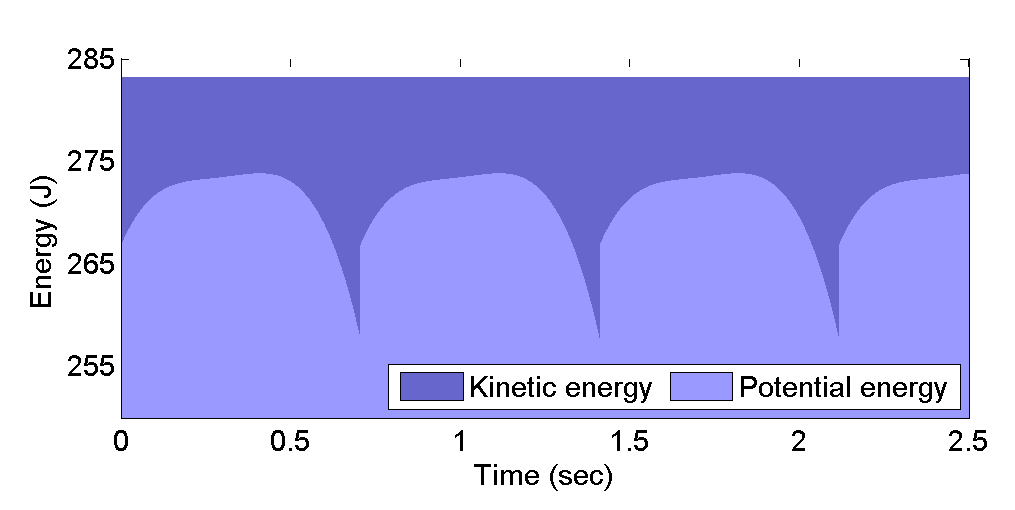
\includegraphics[width=1.0\columnwidth]{energy_cg2d_slope_model}
      \caption{Energy of the shaped system is conserved.}
    \end{figure}    
  }
  %  \only<3>{
  %    \includemedia[
  %      width=1.0\columnwidth,
  %      height=0.5625\columnwidth,
  %      addresource=amber2d.mp4,
  %      activate=pageopen,
  %      flashvars={source=amber2d.mp4&loop=true&autoPlay=true}
  %    ]{}{}%VPlayer9.swf}
  %  }

  \only<3>{
    Energy shaping can be achieved using:
    \begin{align*}
      \argmin_{u \in \Rn}  \, &\uu^{T} \uu\\
      \mbox{s.t. } & \Aclf\argsqdq \uu \leq \bclf\argsqdq
    \end{align*}
    where
    \begin{align*}
      \Aclf = 2 \eta \Lie{\xgbar} \eta, &&
      \bclf = -\resclfparam \eta^{2} - 2\eta \Lie{\xfbar} \eta,
    \end{align*}
    with
    \begin{align*}
      \eta = \Tnrg\argsqdq + \Unrg(\Psi\argsq) - \Eref.
    \end{align*}
  }

  \only<4>{
    \begin{figure}
      \centering
      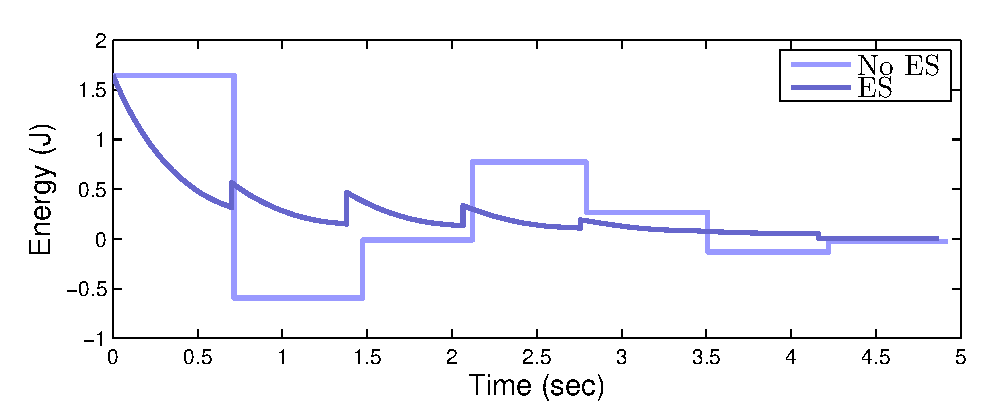
\includegraphics[width=1.0\columnwidth]{es_comparison_2link_conservative}
      \caption{Demonstration of energy shaping on 2-link biped.}
    \end{figure}
  }

  \only<5>{
    \begin{figure}
      \centering
      \includemedia[
        %width=1.0\columnwidth,
        %height=0.5625\columnwidth,
        width=1.0\columnwidth,
        height=0.5\columnwidth,
        addresource=cg2d_es.mp4,
        activate=pageopen,
        flashvars={source=cg2d_es.mp4&loop=true&autoPlay=true}
      ]{}{VPlayer9.swf}
      \caption{Energy shaping to stabilize to a gait from distant initial condition.}
    \end{figure}
  }

  \only<6> {
    \begin{figure}
      \centering
      \subfloat[Nominal system.]{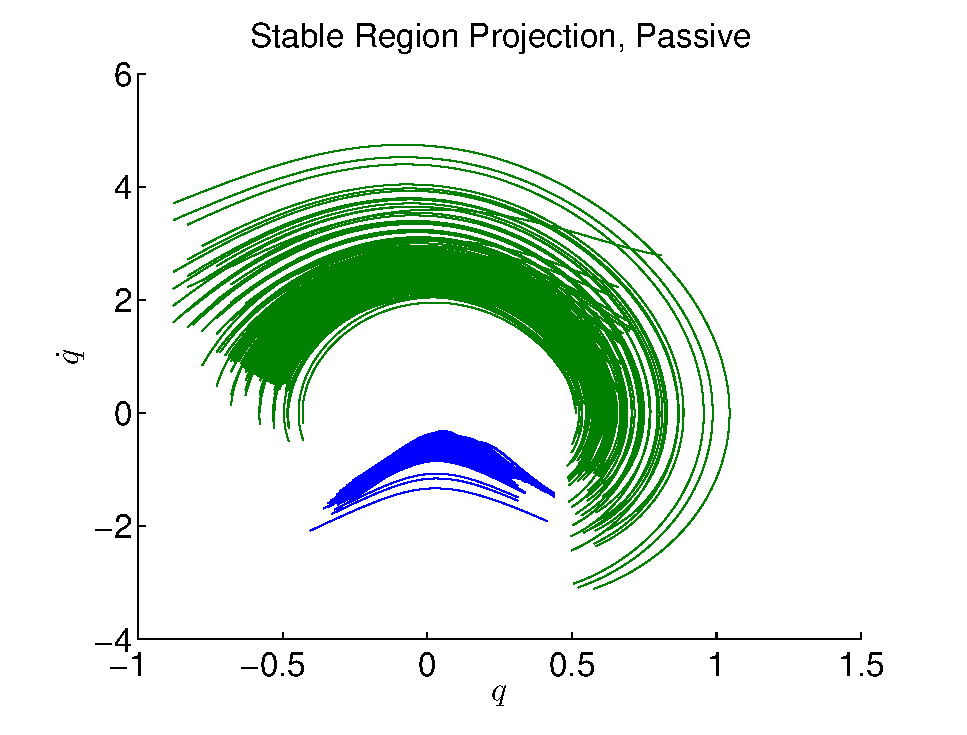
\includegraphics[width=.48\textwidth]{pp_eps_0}}
      \subfloat[Shaped system with $\resclfparam =
      \frac{1}{100}$.]{\includegraphics[width=.48\textwidth]{pp_eps_1_100}}
      \caption{Comparison of unshaped and shaped systems.}
    \end{figure}
  }

  \only<7> {
    \begin{figure}
      \centering
      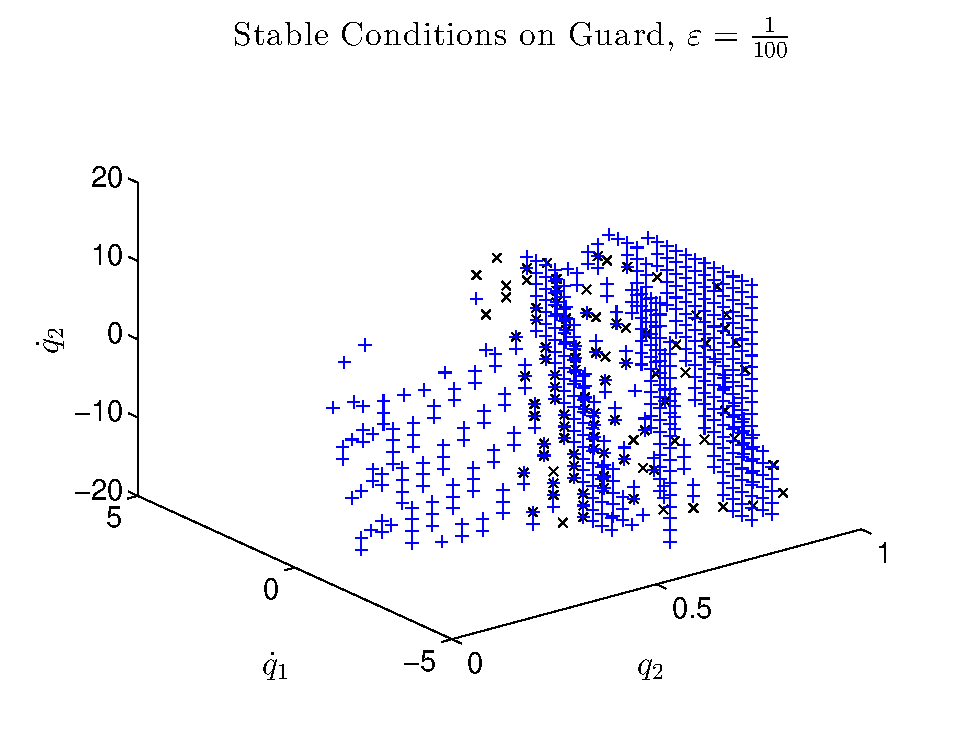
\includegraphics[height=.65\textheight]{poincare_cloud}
      \caption{A three-dimensional representation of the domain of attraction
        on the guard, comparing the unshaped and shaped system.}
    \end{figure}
  }
\end{frame}

\begin{frame}
  \frametitle{Example: 3-Link Biped}
  \only<1>{
    \begin{columns}
      \column{1.5in}
      Dynamic Model:
      \begin{align*}
        \M\argsq \ddq + \CG\argsqdq = \B\argsq \uu
      \end{align*}
      Control Law:
      \begin{align*}
        \vv\argsq& = \G\argsq - \G(\Psi\argsq)\\
        \vv_3\argsq& \ \  +\!= \ -\ck_{d} (\dot \vartheta_{T}^{a}\argsq)\\
        &\hspace{3.2em} -\ck_{p} (\vartheta_{T}^{a}\argsq - \vartheta_{T}^{d}\argsq)
      \end{align*}
      \column{1.5in}
      \begin{figure}
        \centering
        \def\svgwidth{1.0\columnwidth}
        \input{cg2d-3link-model.eps_latex}
        \vspace{-2em}
        \caption{3-link biped configuration.}
      \end{figure}
    \end{columns}
  }
  \only<2>{
    \begin{figure}
      \centering
      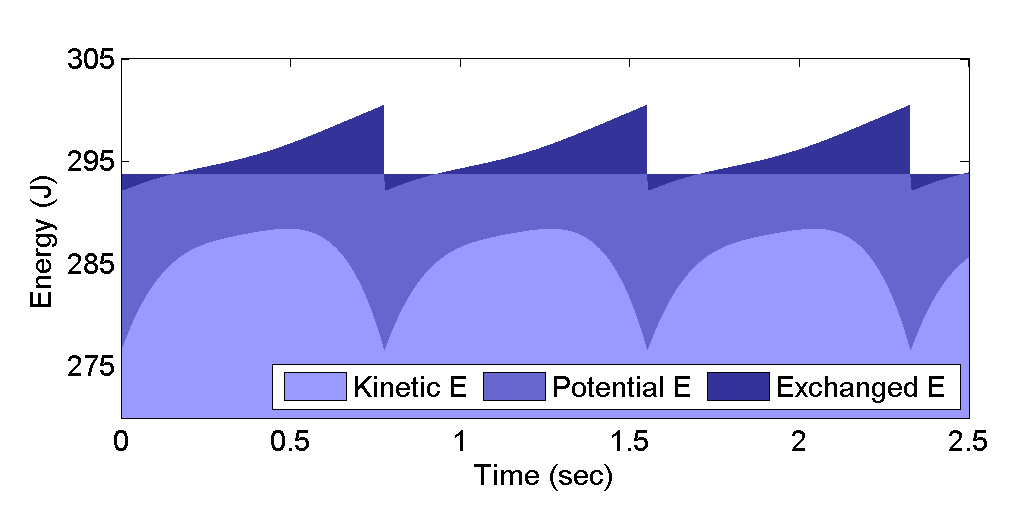
\includegraphics[width=1.0\columnwidth]{energy_conserved_cg2d_3link}
      \caption{The quantity $\Ec\argsqdqW = \Tnrg\argsqdq + \Unrg\argsq -
        \int_{0}^{t} \wrench_{\nc} \cdot \frac{d\q}{d\tau} d\tau$ is
        conserved.}
    \end{figure}
  }
  \only<3>{
    \begin{figure}
      \centering
      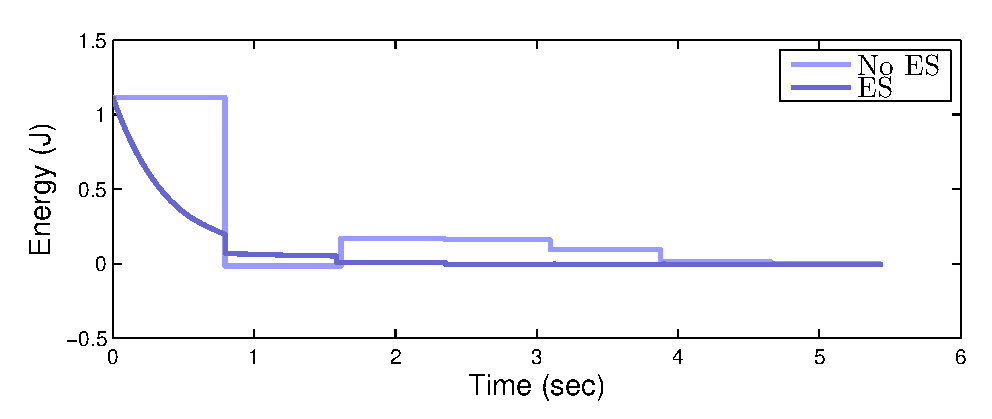
\includegraphics[width=1.0\columnwidth]{es_comparison_3link}
      \caption{Demonstration of energy shaping on 3-link biped.}
    \end{figure}
  }


  \only<4>{
    \begin{figure}
      \centering
      \includemedia[
        %width=1.0\columnwidth,
        %height=0.5625\columnwidth,
        width=1.0\columnwidth,
        height=0.5\columnwidth,
        addresource=3link_es.mp4,
        activate=pageopen,
        flashvars={source=3link_es.mp4&loop=true&autoPlay=true}
      ]{}{VPlayer9.swf}
      \caption{Energy shaping to stabilize to a gait from distant initial condition.}
    \end{figure}
  }

\end{frame}

\begin{frame}
  \frametitle{Multi-Domain Hybrid Systems}
  \begin{itemize}
  \item Complex hybrid systems are made by stitching together domains.
  \item Conserved energy is unique to each domain, i.e.,
    \begin{align*}
      \Ez^{1} \to \Ez^{2} \to \cdots \to \Ez^{n-1} \to \Ez^{n} \to \Ez^{1} \to \cdots
    \end{align*}
  \item Each domain shapes to a specific conserved energy level.
  \end{itemize}
\end{frame}


\begin{frame}
  \frametitle{Example: 7-Link Biped with Feet}
  \only<1>{
    \blue{Appeared in {\bf Automatica}, Aug. 2014}
    \begin{columns}
      \column{1.5in}
      Dynamic Model:
      \begin{align*}
        \M\argsq \ddq + \CG\argsqdq = J^{T}\argsq \lambda + \B\argsq \uu
      \end{align*}
      \column{1.5in}
      \begin{figure}
        \centering
        \def\svgwidth{1.0\columnwidth}
        \input{cg2d-7link-model.eps_latex}
        \vspace{-2em}
        \caption{7-link biped configuration.}
      \end{figure}
    \end{columns}
  }

  \only<2>{
    \begin{block}{Spring--Damper Controller}
      \begin{align*}
        \vv_{\mathit{SD}}\argsq = -\beta e^{-\rho \, h_{\nst}\argsq}
      \end{align*}
      where $\beta, \rho \in \Rpd$ and $h_{\nst} : \Q \to \R$ is the height of the Nonstance toe.
      Used on
      \begin{itemize}
      \item Stance ankle\\
      \item Nonstance ankle\\
      \item Absolute torso angle\\
      \item Non-stance knee spring (only in double support)
      \end{itemize}
      \blue{Provides passivity-based control and toe-off.}
    \end{block}
  }

  \only<3>{
    \begin{block}{Scuffing Prevention Controller}
      \begin{align*}
        \vv_{\mathit{SP}}\argsq = \ck_{p} \theta\argsq - \ck_{d} \dot \theta\argsqdq
      \end{align*}
      where $\ck_{p}, \ck_{d} \in \Rpd$. Used on
      \begin{itemize}
      \item Nonstance ankle
      \end{itemize}
      \blue{Prevents the nonstance toe from colliding with the ground prematurely.}
    \end{block}
  }

\only<4>{
  \begin{figure}
    \centering
      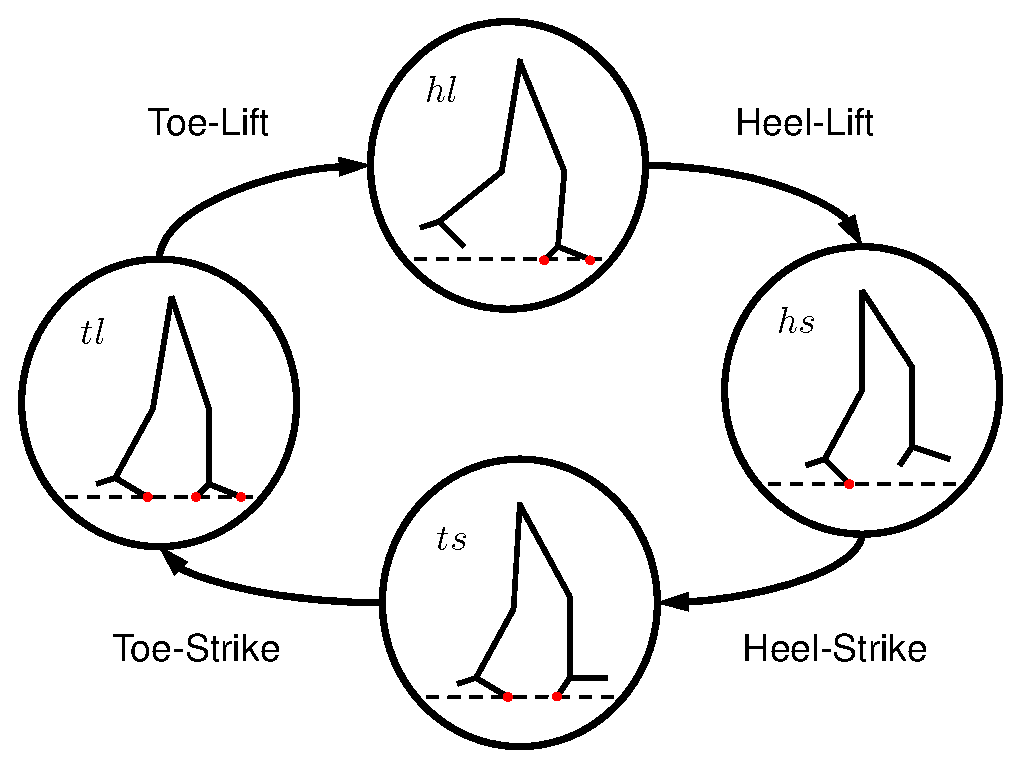
\includegraphics[height=.7\textheight]{domaingraph}
      \caption{The resulting gait traverses a four-domain directed graph.}
    \end{figure}
  }

  \only<5>{
    \begin{figure}
      \centering
      \includemedia[
        %width=1.0\columnwidth,
        %height=0.5625\columnwidth,
        width=1.0\columnwidth,
        height=0.5\columnwidth,
        addresource=7link_es.mp4,
        activate=pageopen,
        flashvars={source=7link_es.mp4&loop=true&autoPlay=true}
      ]{}{VPlayer9.swf}
      \caption{Energy shaping to stabilize to a gait.}
    \end{figure}
  }

  \only<6>{
    \begin{figure}
      \centering
      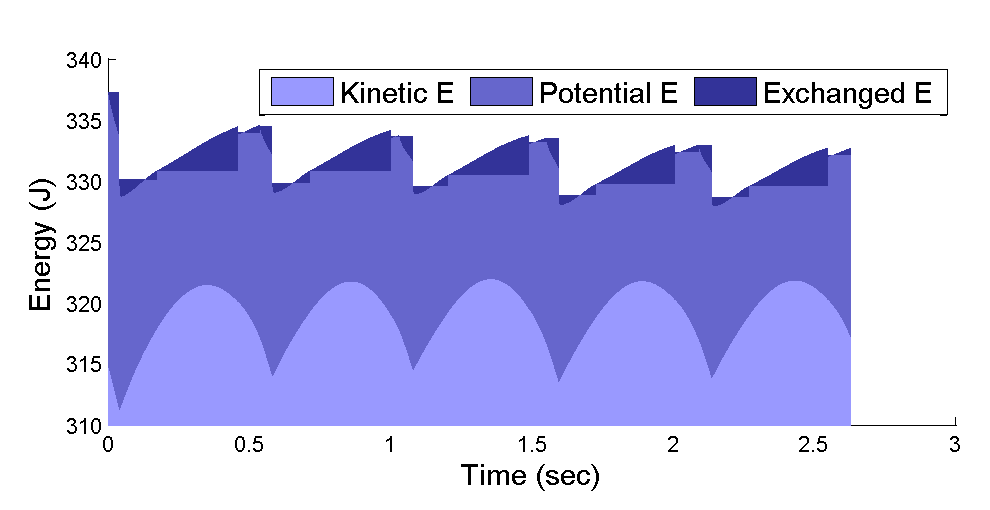
\includegraphics[width=1.0\columnwidth]{energy_conserved_7link}
      \caption{The quantity $\Ez \equiv \Tnrg\argsqdq + \Unrg\argsq -
        \int_{0}^{t} \wrench_{\nc} \cdot \frac{d\q}{d\tau} d\tau$ is
        conserved.}
    \end{figure}
  }

  \only<7>{
    \begin{figure}
      \centering
      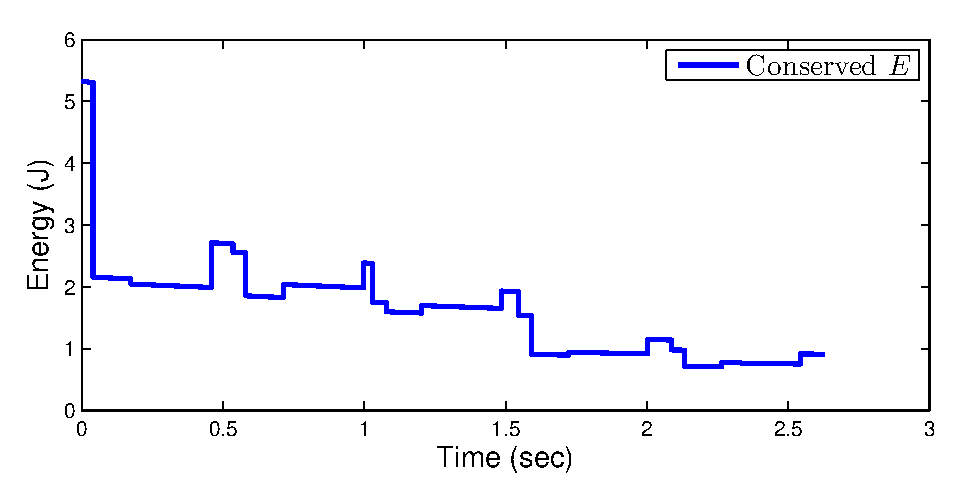
\includegraphics[width=1.0\columnwidth]{energy_conserved_7link_outline}
      \caption{The quantity $\Ez \equiv \Tnrg\argsqdq + \Unrg\argsq -
        \int_{t_0}^{t} \wrench_{\nc} \cdot \frac{d\q}{d\tau} d\tau$ is
        conserved.}
    \end{figure}
  }
  \only<8>{
    \begin{figure}
      \centering
      \includemedia[
        %width=1.0\columnwidth,
        %height=0.5625\columnwidth,
        width=1.0\columnwidth,
        height=0.5\columnwidth,
        addresource=7link_noes.mp4,
        activate=pageopen,
        flashvars={source=7link_noes.mp4&loop=true&autoPlay=true}
      ]{}{VPlayer9.swf}
      \caption{Many steps on the limit cycle.}
    \end{figure}
  }
\end{frame}

\section{Conclusion}
\showtoc

\begin{frame}[t]
  \frametitle{Summary}
  \begin{itemize}
  \item Previous results on total energy shaping lacked a formal proof of
    stability.
  \item Energy shaping can be used to add robustness to hybrid mechanical
    systems.
  \item The limiting behavior of the original system and controller is
    maintained.
  \item It has been shown formally that stability is maintained for small enough
    control gains.
  \end{itemize}
\end{frame}

\begin{frame}
  \centering
  \LARGE{Thank you. Questions?}\\[0em]
  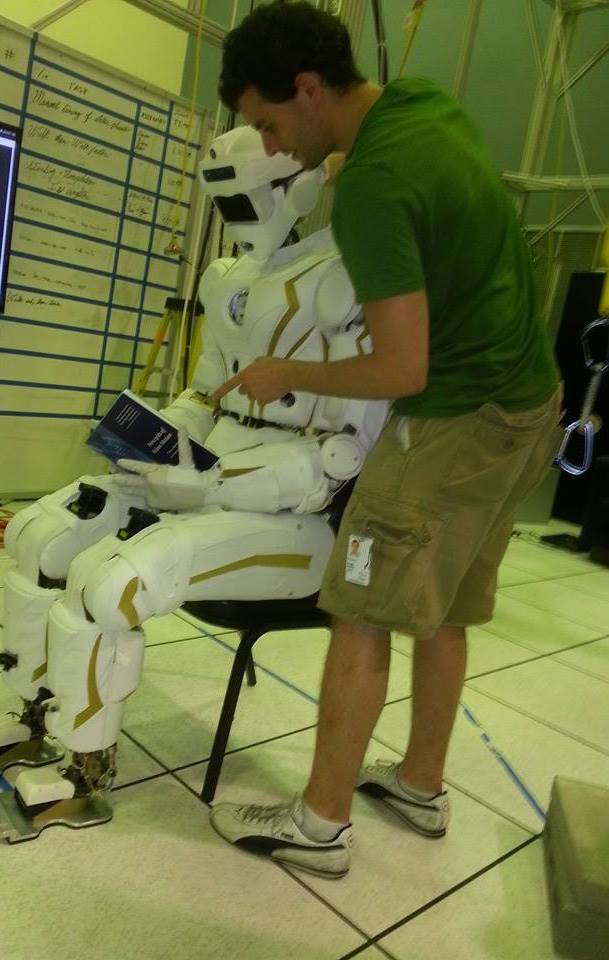
\includegraphics[height=.8\textheight]{sinnet_valkyrie}
\end{frame}


\end{document}
